% !TEX root = ../main.tex
\part{Prolog}

\chapter{Strategie non informate}
In questo capitolo verrà trattata l' implementazione delle due strategie non informate viste a lezione ovvero la ricerca in ampiezza e la ricerca in profondità; per ognuna di queste strategie verrà proposta l'implementazione generale e l'applicazione specifica per due domini che sono il dominio dei cammini e il dominio del mondo dei blocchi.

\section{Ricerca in ampiezza}

\subsection{Il codice sviluppato}
\begin{lstlisting}
ric_amp([nodo(S,LISTA_AZ)|_],LISTA_AZ):- finale(S).
ric_amp([nodo(S,LISTA_AZ)|RESTO],SOL):-
        num_nodi_open,
        espandi(nodo(S,LISTA_AZ),LISTA_SUCC),
        append(RESTO,LISTA_SUCC,CODA),
        ric_amp(CODA,SOL).


espandi(nodo(S,LISTA_AZ),LISTA_SUCC):-
        findall(AZ,applicabile(AZ,S),AZIONI),

        successori(nodo(S,LISTA_AZ),AZIONI,LISTA_SUCC).

successori(_,[],[]).
successori(nodo(S,LISTA_AZ),[AZ|RESTO],[nodo(NUOVO_S,NUOVA_LISTA_AZ)|ALTRI]):-
        trasforma(AZ,S,NUOVO_S),
        append(LISTA_AZ,[AZ],NUOVA_LISTA_AZ),
        successori(nodo(S,LISTA_AZ),RESTO,ALTRI).

num_nodi_open:-
        nb_getval(counter, N1),
        New1 is N1 + 1,
        nb_setval(counter, New1).


ampiezza:- iniziale(S),
        nb_setval(counter , 0),
        ric_amp([nodo(S,[])],SOL),
        writeln(SOL),
        write(N_res).
\end{lstlisting}

\subsection{Analisi dettagliata della strategia}

La ricerca in ampiezza è stata implementata in modo classico, fornendo una regola \lstinline{ric_amp([nodo(S,LISTA_AZ)|_],LISTA_AZ)} per il caso base e una \lstinline{ric_amp([nodo(S,LISTA_AZ)|RESTO],SOL)} per il caso generico.
La prima non fa altro che controllare che lo stato S sia lo stato finale, mentre la seconda invoca le regole \lstinline{ espandi(nodo(S,LISTA_AZ),LISTA_SUCC) } e \lstinline{append(RESTO, LISTA_SUCC,CODA)}, per poi richiamare ricorsivamente \lstinline{ric_amp}.
La regola espandi non fa altro che prendere lo stato \lstinline{S}, espanderlo e cercare tutte le azioni applicabili(con \lstinline{findall} da quello stato; tramite la regola \lstinline{successori()} costruisce la lista dei nuovi stati disponibili a partire dallo stato \lstinline{S}, che saranno poi aggiunti agli stati ancora da espandere tramite la regola \lstinline{append()}.
Infine richiama ricorsivamente la regola per controllare di aver raggiunto lo stato finale e in caso contrario proseguire con l'espansione dei nodi.
Dato che vengono espansi tutti i nodi e dato che un nodo può essere espanso più volte questa strategia può non terminare, perchè fa raggiungere il limite di memoria disponibile.

\subsection{Dominio dei Cammini}
Per quanto riguarda il dominio dei cammini, la ricerca in ampiezza risulta sensata solo se la soluzione si trova ad un livello di profondità relativamente basso, altrimenti si incorre nell'esaurimento di memoria. Per quanto riguarda l'esempio specifico fornito dal Prof. Martelli e quello del professor Torasso la ricerca della soluzione ha esito negativo perchè la soluzione si trova ad un livello di profondità che la ricerca in ampiezza non è in grado di raggiungere.

\subsection{Dominio del Mondo Dei Blocchi}
Anche per quanto riguarda il dominio del mondo dei blocchi il risultato non cambia. Infatti anche in questo caso l'esempio fornito dal professore ha esito negativo perchè nuovamente la soluzione risulta troppo in profondità per essere raggiunta.
\newpage
\section{Ricerca in ampiezza su grafi}

\subsection{Il codice sviluppato}

\begin{lstlisting}
ampiezza :-
    iniziale(S),
    finale(Goal),
    nb_setval(counter , 0),
    time(ric_ampiezza([nodo(S, [])], [], Ris)),
    writeln(Ris),
    nb_getval(counter, N_res),
    write(N_res).


ric_ampiezza([nodo(S, Lista_Az)|_], _, Lista_Az) :- finale(S), !.
ric_ampiezza([nodo(S, Lista_Az) | R_lista_open], Closed, Lista_Ris) :-
        member(S, Closed) ->
        	ric_ampiezza(R_lista_open, Closed, Lista_Ris);
        num_nodi_open,
        open_node(nodo(S, Lista_Az), Lista_children),
        ord_union(Lista_children, R_lista_open, Nuova_open),
        ric_ampiezza(Nuova_open,[S|Closed], Lista_Ris).

open_node(nodo(S, Lista_Az), Lista_childern) :-
        findall(Az, applicabile(Az,S), Az_applicabili),
        node(nodo(S, Lista_Az), Az_applicabili, Lista_childern).

num_nodi_open:-
        nb_getval(counter, N1),
        New1 is N1 + 1,
        nb_setval(counter, New1).

node(_,[],[]).
node(nodo(S, Lista_Az), [Az|R_az], Lista_children) :-
        finale(Goal),
        trasforma(Az, S, Nuovo_S),
        append(Lista_Az, [Az], Nuova_lista_az),
        node(nodo(S, Lista_Az), R_az, Old_children),
        ord_add_element(Old_children, nodo(Nuovo_S, Nuova_lista_az), Lista_children).
\end{lstlisting}

\subsection{Analisi dettagliata della strategia}

La ricerca in ampiezza su grafi può essere considerata come un ottimizzazione della ricerca in ampiezza classica. Introduce il concetto di lista chiusa per migliorare la ricerca della soluzione. Una lista chiusa non è altro che una lista composta da tutti i nodi visitati. Quando
dobbiamo espandere un nuovo nodo andiamo prima a verificare che questo nodo non sia nella lista dei nodi chiusi (nel codice con \lstinline{member(S, Closed) -> ric_ampiezza(R_lista_open, Closed, Lista_Ris);}); se appartiene a quella lista lo scartiamo semplicemente, se invece non appartiene a quella lista allora possiamo procedere con l'espansione con la regola  \lstinline{open_node(nodo(S, Lista_Az), Lista_children),}.
Evitando di ri-espandere nodi già completamente visitati migliora di molto la versione base dell'algoritmo della visita in ampiezza, riducendo di molto il numero di nodi che vengono effettivamente visitati. Una volta aperto il nodo non si fa altro che verificare tutte le azioni applicabili da quel nodo \lstinline{findall(Az, applicabile(Az,S), Az_applicabili),}, dopodiche si invoca la regola \lstinline{node(nodo(S, Lista_Az), Az_applicabili, Lista_childern)} che non fa altro che applicare le azioni prese dalla lista delle azioni possibile ed inserire i nodi risultanti nei nodi da visitare ai passi successivi.

\subsection{Dominio dei Cammini}
Vista l'ottimizzazione apportata all'algoritmo di base per la ricerca in ampiezza, il nuovo algoritmo è in grado di trovare una soluzione agli esempi presi in esame precedentemente con la sola ricerca in ampiezza. Nello specifico sull'esempio del professor Martelli (cammini 10x10) l'algoritmo trova una soluzione in 0.017 secondi, visitando appena 66 nodi e facendo 19508 inferenze. Si è riusciti a passare dalla non terminazione ad avere una soluzione con appena 66 nodi visitati. Anche per quanto riguarda l'esempio del professor Torasso (cammini 20x20) l'algoritmo è in grado di trovare una soluzione in 0.031 secondi, visitando 374 nodi e facendo 178644 inferenze. Anche in questo caso abbiamo un aumento impressionante delle prestazioni, dato che ovviamente nella versione di base non era in grado di generare una soluzione.
Qui di seguito abbiamo i grafici riassuntivi dei risultati ottenuti.

\begin{figure}[htp]
  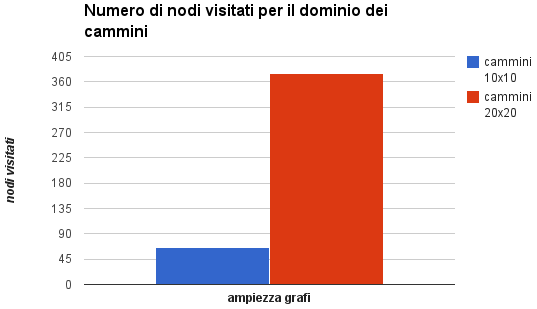
\includegraphics[width=\textwidth]{nodi_visitati_amp_grafi_cammini.png}
  \caption{Nodi visitati per i domini dei cammini}
  \label{fig:figure1}
\end{figure}

\begin{figure}[htp]
  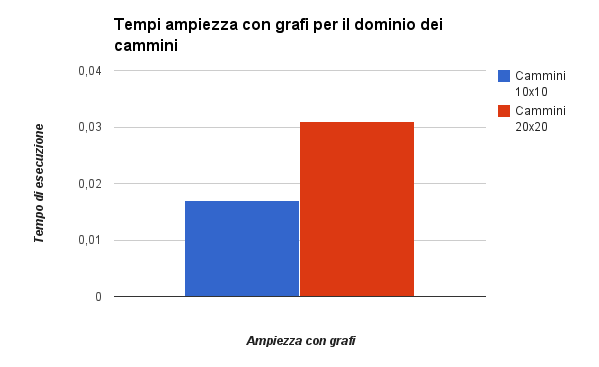
\includegraphics[width=\textwidth]{tempi_amp_grafi_cammini.png}
  \caption{Tempi di calcolo per i domini dei cammini}
  \label{fig:figure2}
\end{figure}

\subsection{Dominio del Mondo Dei Blocchi}
Anche in questo caso la strategia è in grado di fornirci una soluzione a differenza della controparte di base. Per quanto riguarda l'esempio fornito dal professor Martelli l'algoritmo è in grado di generare una soluzione in 0.085 secondi, visitando 487 nodi e facendo 528177 inferenze.Sfortunatamente per quanto riguarda l'esempio del professor Torasso la situazione non cambia dalla versione base; l'algoritmo non è in grado di trovare la soluzione e Prolog ci ritorna out of memory che indica che il limite di memoria è stato raggiunto.
Qui di seguito abbiamo i grafici riassuntivi dei risultati ottenuti.

\begin{figure}[htp]
  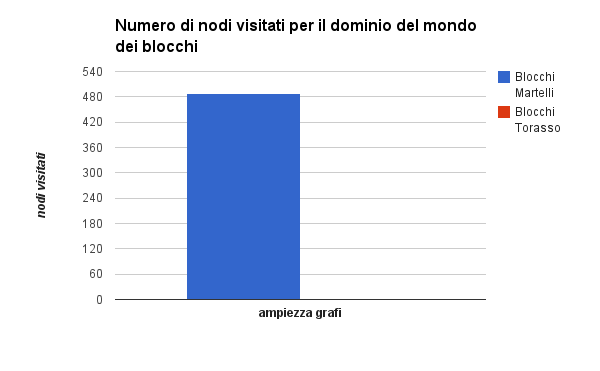
\includegraphics[width=\textwidth]{nodi_visitati_amp_grafi_blocchi.png}
  \caption{Nodi visitati per i domini del mondo dei blocchi}
  \label{fig:figure3}
\end{figure}

\begin{figure}[htp]
  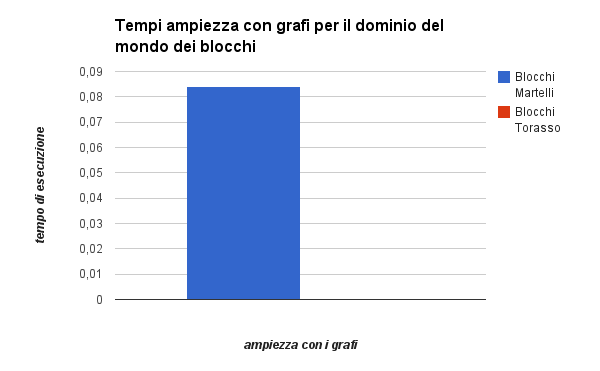
\includegraphics[width=\textwidth]{tempi_amp_grafi_blocchi.png}
  \caption{Tempi di calcolo per i domini del mondo dei blocchi}
  \label{fig:figure4}
\end{figure}
\newpage
\section{Ricerca in profondità}

\subsection{Il codice sviluppato}

\begin{lstlisting}
ric_prof_cc_lim(S,_,_,[]) :- finale(S),!.
ric_prof_cc_lim(S,D,Visitati,[Az|Resto]) :-
    D>0,
    applicabile(Az,S),
    trasforma(Az,S,Nuovo_S),
    \+ member(Nuovo_S,Visitati),
    num_nodi_open,
    D1 is D-1,
    ric_prof_cc_lim(Nuovo_S,D1,[S|Visitati],Resto).

ric_prof_cc_id(I,D,Ris) :- ric_prof_cc_lim(I,D,[],Ris).
ric_prof_cc_id(I,D,Ris) :-
    D1 is D+1,
    ric_prof_cc_id(I,D1,Ris).

num_nodi_open:-
        nb_getval(counter, N1),
        New1 is N1 + 1,
        nb_setval(counter, New1).

prof_lim(D) :- iniziale(I),ric_prof_cc_lim(I,D,[],Ris),write(Ris).
prof_id :-
        iniziale(I),
        nb_setval(counter , 0),
        time(ric_prof_cc_id(I,1,Ris)),
        nb_getval(counter, N_res),
        writeln(Ris),
        write(N_res),
        write('\n').
\end{lstlisting}

\subsection{Analisi dettagliata della strategia}

La ricerca in profondità è stato sviluppata in 2 versione; la prima riceve in input una profondità D oltre la quale la ricerca non può andare; la seconda invece parte con una profondità di 1 e man mano che vengono visitati tutti i nodi entro quella profondità senza trovare soluzione, la profondità viene aumentata di un livello. La seconda procedura è denominata Iterative Deepening.
L'implementazione della prima versione è molto semplice. Come per la ricerca in ampiezza abbiamo 2 regole, una per il caso base e una per il caso generico. Nuovamente la regola per il caso base non fa altro che verificare che lo stato corrente \lstinline{S} sia lo stato finale. La regola del passo generico è stata sviluppata nel seguente modo: se la profondità non è minore di zero applico allo stato corrente S la prima delle azioni applicabili disponibili, dopodiche controllo che il nuovo stato non sia stato già visitato, decremento la profondità di 1 ed infine richiamo la regola ricorsivamente sul nuovo stato. Se la profondità risulta minore di zero, significa che ho superato il limite imposto e di conseguenza non posso scendere oltre nell'espansione.
Prolog farà backtracking e procederà con l'applicazione di un'altra delle azioni applicabili per quel nodo e si procede nuovamente come descritto sopra. Se la soluzione è oltre il limite imposto a priori Prolog resituirà false, altrimenti viene restituita la lista delle azioni per raggiungerla.
L'implementazione della seconda versione sfrutta la prima. Utilizza le due regole per scendere in profondità nei vari stati, ai quali viene aggiunta una regola per aumentare il limite di un livello, quando la ricerca non trova soluzione all'interno del limite corrente. Il limite che viene fornito a priori è di 1 e ci si ferma solo quando si trova la soluzione.


\subsection{Dominio dei Cammini}
A differenza della ricerca in ampiezza, la ricerca a profondità limitata con approfondimento iterativo (iterative deepening) è in grado di fornire una soluzione ottima e di lunghezza minima per i problemi relativi al dominio dei cammini, dato che tutte le azioni relative a questo dominio hanno costo unitario. Per quanto riguarda l'esempio specifico fornito dal Prof. Martelli (cammino 10x10) la ricerca in profondità limitata con approfondimento iterativo è in grado di trovare una delle soluzioni di lunghezza minima (se si hanno più soluzioni con la stessa lunghezza possono essere visualizzate tramite il comando ; dopo la visualizzazione della prima soluzione). La soluzione viene trovata in tempo ragionevole, circa 3.203 secondi con un numero di nodi visitati pari a 548376 e un numero di inferenze pari a 21265407. Per quanto riguarda l'esempio fornito dal professor Torasso (cammino 20x20), la ricerca in profondità impiega un tempo taltmente elevato che ci è stato impossibile verificare la sua terminazione. Le nostre prove sul dominio sono durate 30 e 50 minuti senza riuscire ad ottenere una soluzione, di conseguenza possiamo affermare che non è una strategia ragionevole per risolvere quel determinato esempio.
Qui di seguito abbiamo i grafici riassuntivi dei risultati ottenuti.

\begin{figure}[htp]
  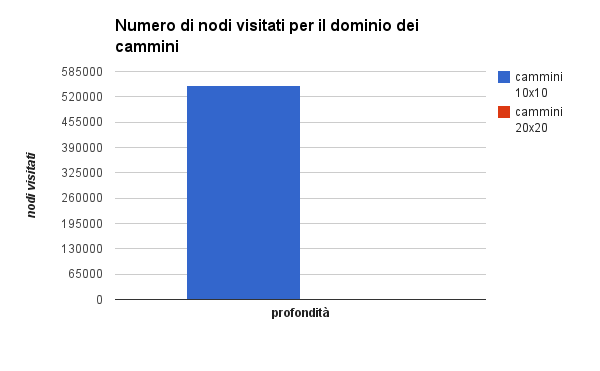
\includegraphics[width=\textwidth]{nodi_visitati_profondita_cammini.png}
  \caption{Nodi visitati per i domini dei cammini}
  \label{fig:figure5}
\end{figure}

\begin{figure}[htp]
  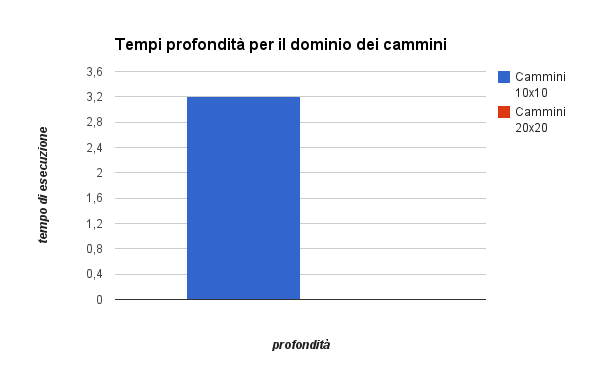
\includegraphics[width=\textwidth]{tempi_prof_cammini.png}
  \caption{Tempi di calcolo per i domini dei cammini}
  \label{fig:figure6}
\end{figure}

\subsection{Dominio del Mondo dei Blocchi}
Anche in questo caso la strategia implementata è in grado di fornire la soluzione ottima a lunghezza minima. Per quanto riguarda l'esempio del professor Martelli l'algoritmo trova soluzione in 0.459 secondi circa, visitando 13222 nodi e facendo 3364820 inferenze. Invece sull'esempio fornito dal professor Torasso l'algoritmo si comporta decisamente peggio ma riesce comunque a trovare la soluzione in un tempo ragionevole che è di 232.268 secondi. Ovviamente visto l'elevato tempo richiesto per trovare la soluzione l'algoritmo ha visitato 4180656 nodi e ha compiuto 1548207210 inferenza.
Qui di seguito abbiamo i grafici riassuntivi dei risultati ottenuti.

\begin{figure}[htp]
  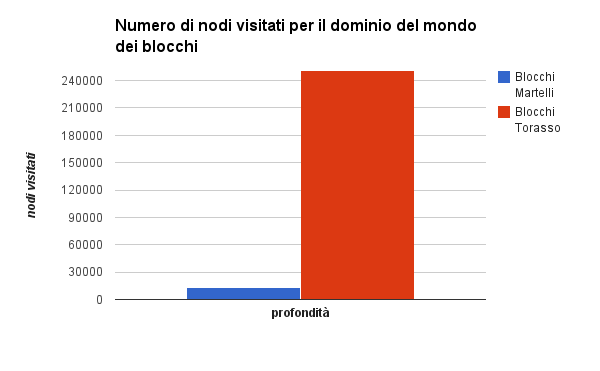
\includegraphics[width=\textwidth]{nodi_visitati_profodnita_blocchi.png}
  \caption{Nodi visitati per i domini del mondo dei blocchi}
  \label{fig:figure7}
\end{figure}

\begin{figure}[htp]
  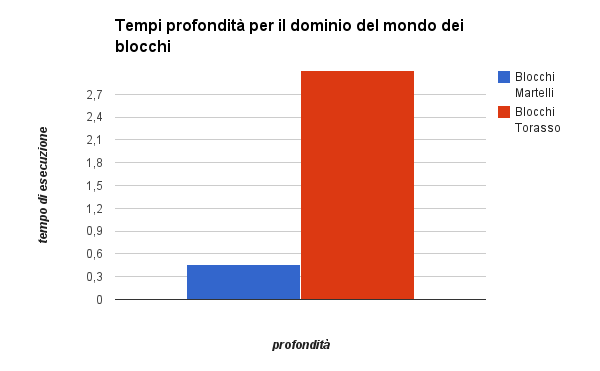
\includegraphics[width=\textwidth]{tempi_prof_blocchi.png}
  \caption{Tempi di calcolo per i domini del mondo dei blocchi}
  \label{fig:figure8}
\end{figure}

\chapter{Strategie informate}
In questo capitolo verrà trattata l'implementazione delle strategie informate viste a lezione ovvero la ricerca in ampiezza sui grafi, la ricerca in profondità ad approfondimento iterativo con stima (IDA*) e la ricerca in ampiezza sui grafi con stima (A*); per ognuna di queste strategie verrà proposta l'implementazione generale e l'euristica specifica utilizzata per i due domini proposti che sono il dominio dei cammini e il dominio del mondo dei blocchi.

\section{Ricerca in profondità ad approfondimento iterativo con stima (IDA*)}

\subsection{Il codice sviluppato}

\begin{lstlisting}
ric_prof_lim(S,Depth,_,_,[]) :-
        f_val(F),
        F =< Depth,
        finale(S),!.
ric_prof_lim(S,Depth,G,Visitati,[Az|Resto]) :-
        f_val(F),
        F =< Depth,
                 applicabile(Az,S),
                 trasforma(Az,S,Nuovo_S),
                 \+ member(Nuovo_S,Visitati),
                 num_nodi_open,
                 G1 is G + 1,
                 calcolo_euristica(Nuovo_S,G1),
                 ric_prof_lim(Nuovo_S,Depth,G1,[S|Visitati],Resto).
ric_prof_lim(_,Depth,_,_,_) :-
        f_val(F),
        F > Depth,
        try_prof(F),
        fail.

try_prof(F) :-
        soglia(X),
        X =< F, !
        ;
        retract(soglia(X)), !,
        assert(soglia(F)).

num_nodi_open:-
        nb_getval(counter, N1),
        New1 is N1 + 1,
        nb_setval(counter, New1).

ric_idastar(I,Ris,Depth,G) :- ric_prof_lim(I,Depth,G,[],Ris).

ric_idastar(I,Ris,_,G) :-
        soglia(Sog),
        retract(soglia(Sog)),
        assert(soglia(99999)),
        ric_idastar(I,Ris,Sog,G).

idastar :-
        iniziale(S),
        nb_setval(counter , 0),
        calcolo_euristica(S,0),
        f_val(D),
        time(ric_idastar(S,Ris,D,0)),
        nb_getval(counter, N_res),
        writeln(Ris),
        write(N_res),
        write('\n').
\end{lstlisting}

\subsection{Analisi dettagliata della strategia}

L'implementazione dell'algoritmo è stata fatta in modo da sfruttare il lavoro già fatto con la ricerca in profondità con approfondimento iterativo, alla quale andiamo ad aggiungere un euristica specifica per ogni dominio che fornirà un valore di soglia per la nostra ricerca in profondità.
La soglia viene inizializzata con un valore di default molto grande, ma man mano che l'esecuzione prosegue, viene sostituita di volta in volta con la \lstinline{f_val} minima presa dai nodi che hanno superato la soglia nell'iterazione precedente.
Più nel dettaglio l'algoritmo inizia il suo lavoro settando la \lstinline{f_val} che verrà utilizzata come limite di ricerca e richiamando la ricerca in profondità già sviluppata precedentemente con alcune piccole modifiche.
Nel caso base è stato aggiunto un controllo sulla profondità, ovvero che la nostra \lstinline{f_val} deve essere minore o uguale alla profondità; se è cosi si procede con il semplice controllo di S come stato finale, altrimenti si passa alla regola per aggiornare la soglia.
Per quanto riguarda il caso generico, abbiamo sempre il controllo della \lstinline{f_val} sulla profondità e in più abbiamo il suo ricalcolo tramite l'euristica specifica del dominio. La regola \lstinline{try_prof(F)} ha una doppia funzione: oltre ad aggiornare la soglia quando questa risulta maggiore della nostra \lstinline{f_val} corrente, ci permette di bloccare la ricerca quando siamo nel caso opposto, ovvero che la \lstinline{f_val} risulta maggiore del nostro valore di soglia fissato. Infine quando la ricerca in profondità fallisce abbiamo una regola per riportare al valore di default la soglia e ricominciare nuovamente la ricerca in profondità.

\subsection{Dominio dei Cammini}

\begin{lstlisting}
calcolo_euristica(pos(R,C),pos(R1,C1), G) :-
        X is R - R1,
        Y is C - C1,
        abs(X, Xabs),
        abs(Y, Yabs),
        H is Xabs + Yabs,
        F is G + H,
        retract(f_val(_)),
        assert(f_val(F)),
        retract(h_val(_)),
        assert(h_val(H)).
\end{lstlisting}

Per quanto riguarda il dominio dei cammini l'euristica utilizzata per generare i valori di \lstinline{f_val} è stata la classica distanza di Manhattan. Vengono presi in inpunt le coordinate \lstinline{x} e \lstinline{y} del nodo corrente e del nodo goal e si esegue questo semplice calcolo:

$$ L1(p1,p2) = |x1 - x2| + |y1 - y2|$$
$$F = G + L1$$

\lstinline{G} viene passata come parametro nella regola, mentre il valore \lstinline{F} che viene calcolato viene asserto come \lstinline{f_val}. Per quanto riguarda l'esempio fornito dal Prof. Martelli (cammini 10x10) l'algoritmo precedentemente descritto, sfruttando quest'euristica, è in grado di fornire la soluzione ottima a costo minimo; nello specifico l'algoritmo fornisce una soluzione dopo 0.123 secondi, visitando solamente 13078 nodi e facendo 681842 inferenze. Anche sull'esempio del professor. Torasso (cammini 20x20) l'algoritmo si comporta egregiamente trovando soluzione in solamente 0.146 secondi, visitando 15796 nodi e facendo 791573 inferenze.
Qui di seguito abbiamo i grafici riassuntivi dei risultati ottenuti.

\begin{figure}[htp]
  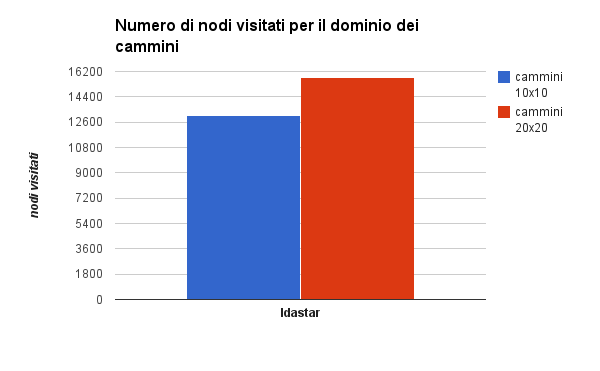
\includegraphics[width=\textwidth]{nodi_visitati_ida_cammini.png}
  \caption{Nodi visitati per i domini dei cammini}
  \label{fig:figure9}
\end{figure}

\begin{figure}[htp]
  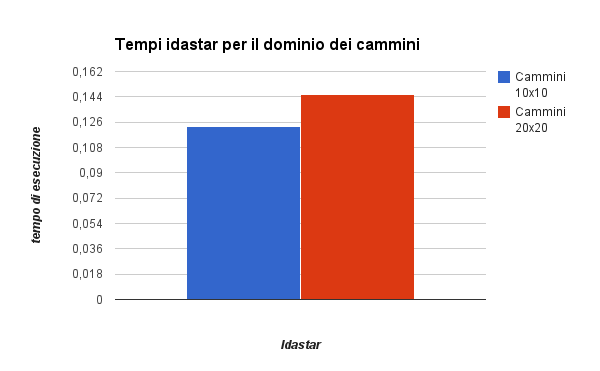
\includegraphics[width=\textwidth]{tempi_ida_cammini.png}
  \caption{Tempi di calcolo per i domini dei cammini}
  \label{fig:figure10}
\end{figure}

\subsection{Dominio del Mondo dei Blocchi}

\begin{lstlisting}
calcolo_euristica(S, G) :-
        goal(Res),
        ord_subtract(S, Res, Diff),
        calcola_h(Diff, Ndiff),
        h_val(Ndiff),
        F is G + Ndiff,
        retract(f_val(_)),
        assert(f_val(F)).

calcola_h([],0).
calcola_h([_|Resto_Ok],H) :-
        calcola_h(Resto_Ok, H1),
        H is H1 + 1,
        retract(h_val(_)),
        assert(h_val(H)).
\end{lstlisting}

L'euristica utilizzata per il mondo dei blocchi fornisce il nostro valore di \lstinline{f_val} sommando il costo del cammino trovato dal nodo iniziale al nodo corrente, con il numero dei blocchi che si trovano nella posizione della configurazione finale. Questo viene fatto generando la lista dei nodi in posizione corretta tramite \lstinline{ord_subtract(List1,List2,Res)}. \lstinline{Ord_subtract} è una regola nativa di Prolog e non fa altro che sottrarre la \lstinline{List1} dalla \lstinline{List2} due e mettere la lista risultante in \lstinline{Res}. Infine tramite la regola \lstinline{calcola_h} contiamo gli elementi di \lstinline{Res} per trovare il numero dei blocchi in posizione correta che saranno poi sommati a G per avere la nostra \lstinline{f_val}. L'algoritmo si dimostra estremamente veloce anche in questo dominio risolvendo l'esempio del professor Martelli in soli 0.076 secondi, visitando appena 1444 nodi e facendo 477443 inferenze. Sull'esempio del professor Torasso si ha un significativo aumento nei tempi di risoluzione, ma l'algoritmo si comporta comunque ottimamente mettendoci 14.564 secondi per trovare la soluzione. Ovviamente tempi maggiori comportano un maggior numero di nodi visitati e di inferenze che in questo caso sono 183364 per quanto riguarda i nodi visitati e 89033213 per quanto riguarda il numero di inferenze eseguite.
Qui di seguito abbiamo i grafici riassuntivi dei risultati ottenuti.

\begin{figure}[htp]
  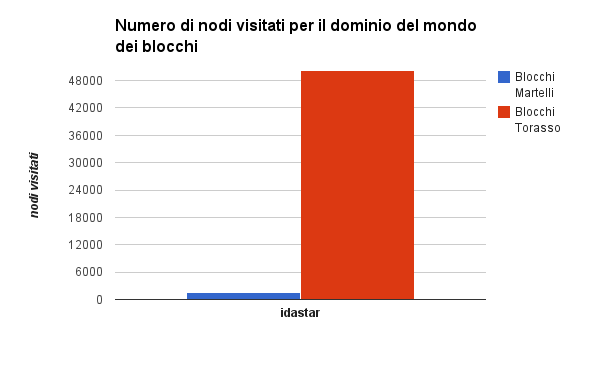
\includegraphics[width=\textwidth]{nodi_visitati_ida_blocchi.png}
  \caption{Nodi visitati per i domini del mondo dei blocchi}
  \label{fig:figure11}
\end{figure}

\begin{figure}[htp]
  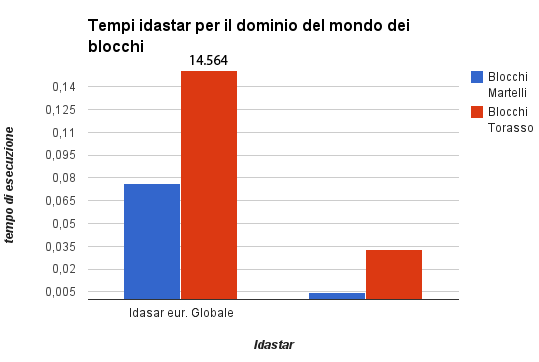
\includegraphics[width=\textwidth]{tempi_ida_blocchi.png}
  \caption{Tempi di calcolo per i domini del mondo dei blocchi}
  \label{fig:figure12}
\end{figure}

\newpage
\section{Ricerca in ampiezza sui grafi con stima (A*)}

\subsection{Il codice sviluppato}

\begin{lstlisting}
ric_astar([nodo(_,_, S, Lista_Az)|_],_, Lista_Az) :- finale(S), !.
ric_astar([nodo(Fcost, Gcost, S, Lista_Az)| R_lista_open], Closed, Lista_Ris) :-
        member(S, Closed) ->
                ric_astar(R_lista_open, Closed, Lista_Ris);
        num_nodi_open,
        open_node(nodo(Fcost, Gcost, S, Lista_Az), Lista_children),
        ord_union(Lista_children, R_lista_open, Nuova_open),
        ric_astar(Nuova_open,[S|Closed],Lista_Ris).

open_node(nodo(Fcost, Gcost, S, Lista_Az), Lista_childern) :-
        findall(Az, applicabile(Az,S), Az_applicabili),
        best_node(nodo(Fcost, Gcost, S, Lista_Az), Az_applicabili, Lista_childern).

best_node(_,[],[]).
best_node(nodo(Fcost, Gcost, S, Lista_Az), [Az|R_az], Lista_children) :-
        trasforma(Az, S, Nuovo_S),
        append(Lista_Az, [Az], Nuova_lista_az),
        % num_nodi_open,
        best_node(nodo(Fcost, Gcost, S, Lista_Az), R_az, Old_children),
        G1 is Gcost + 1,
        calcolo_euristica(Nuovo_S, G1),
        f_val(F),
        ord_add_element(Old_children, nodo(F, G1, Nuovo_S, Nuova_lista_az), Lista_children).

num_nodi_open:-
        nb_getval(counter, N1),
        New1 is N1 + 1,
        nb_setval(counter, New1).

astar :-
        iniziale(S),
        nb_setval(counter , 0),
        calcolo_euristica(S, 0),
        f_val(Fcost),
        time(ric_astar([nodo(Fcost, 0, S, [])], [], Ris)),
        nb_getval(counter, N_res),
        writeln(Ris),
        write(N_res),
        write('\n').
\end{lstlisting}

\subsection{Analisi dettagliata della strategia}

L'implementazione dell'algoritmo di ricerca astar è stato fatto in modo molto semplice. Sfruttando le regole native di Prolog \lstinline{ord_union()} e \lstinline{ord_add_element} possiamo costruire delle liste di nodi ordinate secondo il loro \lstinline{f_val()} cosi da avere la certezza di analizzare sempre lo stato migliore fra quelli all'interno della lista degli stati da visitare. Vediamo più nel dettaglio l'implementazione. Come al solito la ricerca astar è composta di 2 regole principali, una per il caso base che non fa altro che controllare che lo stato in input S sia lo stato finale e una per caso generico. La regola per il caso generico controlla prima di tutto che lo stato in inpunt non faccia parte della lista dei nodi chiusi e quindi già visitato; in caso affermativo, richiamiamo la ricerca astar sul nodo successivo nella lista dei nodi aperti, mentre in caso negativo lo apriamo con la regola \lstinline{open_node()}. La regola non fa altro che cercare tutte le azioni applicabili dal nodo corrente, inserendole in una lista di azioni che verrà data in pasto alla regola \lstinline{best_node()}. La regola \lstinline{best_node()} non fa altro che costruire una lista ordinata di figli basata sul loro \lstinline{f_val()} in ordine crescente.
La costruzione viene fatta grazie a \lstinline{ord_add_element (Set1,Elem,SetRes)} il quale prende in input una lista ordinata di elementi (\lstinline{Set1}) alla quale aggiunge in modo ordinato il nuovo elemento (\lstinline{Elem}) mettendo infine il risultato nella lista ordinata SetRes. \lstinline{Res}Terminata la costruzione di questa lista ordinata di nodi figlio, la aggiungiamo alla lista dei nodi aperti tramite la regola \lstinline{ord_union(Set1,Set2,SetRes)} la quale non fa altro che unire ordinatamente le due liste mettendo nuovamente il risultato in SetRes.
Come ultimo passo richiamiamo la ricerca astar sul primo nodo della lista dei nodi aperti e aggiungiamo il nodo corrente alla lista dei nodi chiusi.

\subsection{Dominio dei Cammini}

\begin{lstlisting}
calcolo_euristica(pos(R,C),pos(R1,C1), G) :-
        X is R - R1,
        Y is C - C1,
        abs(X, Xabs),
        abs(Y, Yabs),
        H is Xabs + Yabs,
        F is G + H,
        retract(f_val(_)),
        assert(f_val(F)),
        retract(h_val(_)),
        assert(h_val(H)).
\end{lstlisting}

Per quanto riguarda il dominio dei cammini è stata utilizzata la stessa euristica descritta per la ricerca ad approfondimento iterativo con stima (IDA*) ovvero la distanza di Manhattan. Con l'esempio del professor Martelli (cammini 10x10) l'algoritmo impiega appena 0.029 secondi per trovare la soluzione; visita appena 53 nodi ed esegue solamente 19517 inferenze per arrivare al goal. Anche con l'esempio del professor Torasso (cammini 20x20) l'algoritmo si comporta ottimamente impiegando 0.037 secondi, visitando 128 nodi e facendo 65057 inferenze per trovare la soluzione.
Qui di seguito abbiamo i grafici riassuntivi dei risultati ottenuti.

\begin{figure}[htp]
  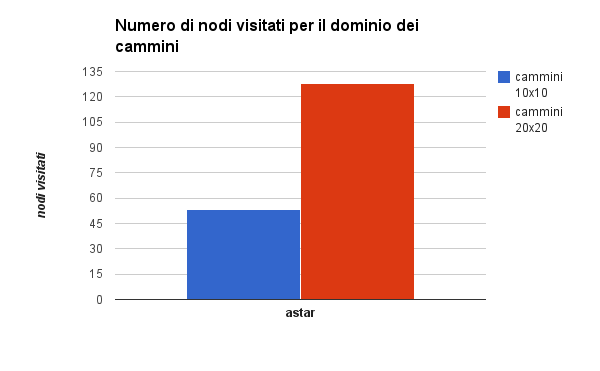
\includegraphics[width=\textwidth]{nodi_visitati_astar_cammini.png}
  \caption{Nodi visitati per i domini dei cammini}
  \label{fig:figure13}
\end{figure}

\begin{figure}[htp]
  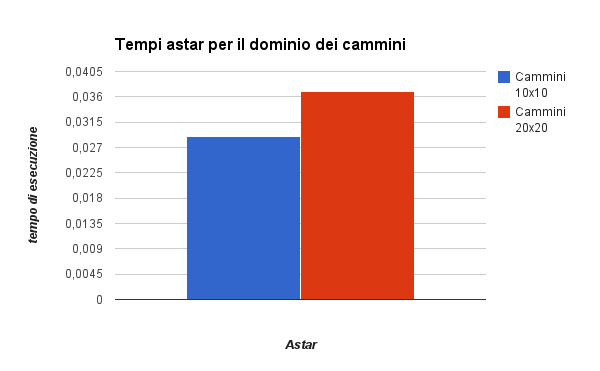
\includegraphics[width=\textwidth]{tempi_astar_cammini.png}
  \caption{Tempi di calcolo per i domini dei cammini}
  \label{fig:figure14}
\end{figure}

\subsection{Dominio del Mondo dei Blocchi}

\begin{lstlisting}
calcolo_euristica(S, G) :-
        goal(Res),
        ord_subtract(S, Res, Diff),
        calcola_h(Diff, Ndiff),
        h_val(Ndiff),
        F is G + Ndiff,
        retract(f_val(_)),
        assert(f_val(F)).

calcola_h([],0).
calcola_h([_|Resto_Ok],H) :-
        calcola_h(Resto_Ok, H1),
        H is H1 + 1,
        retract(h_val(_)),
        assert(h_val(H)).
\end{lstlisting}

Anche per il dominio del mondo dei blocchi l'euristica utilizzata è la stessa della ricerca ad approfondimento iterativo con stima (IDA*), riuscendo anche in questo a fornire una soluzione ottima a costo minimo. Per quanto riguarda l'esempio fornito dal professor Martelli l'algoritmo si comporta bene trovando una soluzione dopo 0.072 secondi appena, visitando 304 nodi e 396947 inferenze fatte.
Per quanto riguarda l'esempio fornito dal professor Torasso l'algoritmo sfortunatamente non è in grado di fornire una soluzione, dato che esaurisce la memoria disponibile per poter fare inferenza.
Qui di seguito abbiamo i grafici riassuntivi dei risultati ottenuti.

\begin{figure}[htp]
  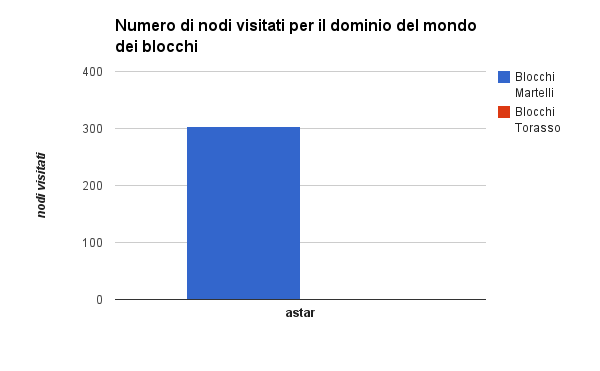
\includegraphics[width=\textwidth]{nodi_visitati_astar_blocchi.png}
  \caption{Nodi visitati per i domini del mondo dei blocchi}
  \label{fig:figure15}
\end{figure}

\begin{figure}[htp]
  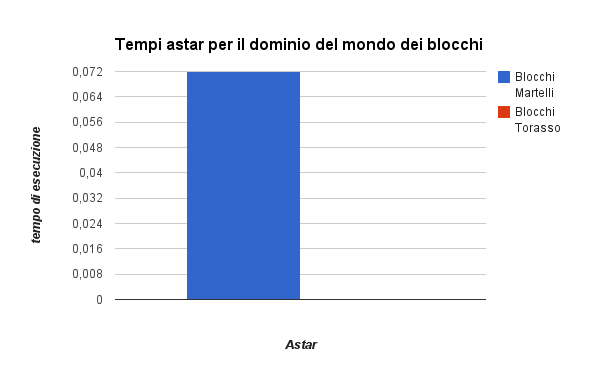
\includegraphics[width=\textwidth]{tempi_astar_blocchi.png}
  \caption{Tempi di calcolo per i domini del mondo dei blocchi}
  \label{fig:figure16}
\end{figure}

\chapter{Metropolitana di Londra}

\section{Il codice sviluppato}

\begin{lstlisting}
calcolo_euristica([at(Stazione1),_],[at(Stazione2),_]) :-
        stazione(Stazione1, R, C),
        stazione(Stazione2, R1, C1),
        X is (R - R1)^2,
        Y is (C - C1)^2,
        abs(X, Xabs),
        abs(Y, Yabs),
        H is Xabs + Yabs,
        F is sqrt(H),
        retract(f_val(_)),
        assert(f_val(F)),
        retract(h_val(_)),
        assert(h_val(H)).

ric_astar([nodo(_,_, S, Lista_Az)|_],_, Lista_Az) :- finale(S), !.
ric_astar([nodo(Fcost, Gcost, S, Lista_Az)| R_lista_open], Closed, Lista_Ris) :-
        member(S, Closed) ->
                ric_astar(R_lista_open, Closed, Lista_Ris);
        num_nodi_open,
        open_node(nodo(Fcost, Gcost, S, Lista_Az), Lista_children),
        ord_union(Lista_children, R_lista_open, Nuova_open),
        ric_astar(Nuova_open,[S|Closed], Lista_Ris).


open_node(nodo(Fcost, Gcost, S, Lista_Az), Lista_childern) :-
        findall(Az, applicabile(Az,S), Az_applicabili),
        best_node(nodo(Fcost, Gcost, S, Lista_Az), Az_applicabili, Lista_childern).

best_node(_,[],[]).
best_node(nodo(Fcost, Gcost, S, Lista_Az), [Az|R_az], Lista_children) :-
        finale(Goal),
        trasforma(Az, S, Nuovo_S),
        append(Lista_Az, [Az], Nuova_lista_az),
        % num_nodi_open,
        best_node(nodo(Fcost, Gcost, S, Lista_Az), R_az, Old_children),
        calcola_G(Az, Gcost, G1),
        calcolo_euristica(Nuovo_S, Goal),
        f_val(F),
        ord_add_element(Old_children, nodo(F, G1, Nuovo_S, Nuova_lista_az), Lista_children).

num_nodi_open:-
        nb_getval(counter, N1),
        New1 is N1 + 1,
        nb_setval(counter, New1).

calcola_G(sali(_,_), Gcost, G1) :-
        G1 is Gcost + 10.

calcola_G(scendi(_), Gcost, G1) :-
        G1 is Gcost + 10.

calcola_G(vai(_,_,_,_), Gcost, G1) :-
        G1 is Gcost + 5.

astar :-
        iniziale(S),
        nb_setval(counter , 0),
        time(ric_astar([nodo(0, 0, S, [])], [], Ris)),
        nb_getval(counter, N_res),
        writeln(Ris),
        write(N_res),
        write('\n').
\end{lstlisting}

\section{Analisi dettagliata della strategia}

Il dominio della metropolitana di Londra risulta leggermente differente dai due domini presi in esame precedentemente, perchè le azioni non hanno un costo unitario. Oltre a dover sviluppare un euristica adatta a calcolare un \lstinline{f_val()} per poter eseguire la ricerca, bisogna anche far fronte che non basta più un semplice incremento di uno del nostro \lstinline{g_val} dopo ogni azione, ma serve un incremento diverso in base all'azione che stiamo per intraprendere. Si è deciso quindi di dare 2 valori di incremento differenti al \lstinline{g_val}: +10 per le azioni di sali/scendi dalla metropolitana e un +5 per le azioni di vai. Con questi pesi le azioni di sali/scendi risultano molto più costose dell'azione di vai, facendo prediligere quindi percorsi più lunghi con pochi cambi di metro a percorsi più brevi ma con cambi più frequenti.
Per quanto riguarda l'euristica scelta si è optati per una semplice distanza euclidea, visto che venivano fornite le coordinate delle stazioni. La distanza euclidea viene calcolata come segue:

$$L1(p1,p2) = sqrt((x1 - x2)+(y1 - y2))$$

Il risultato di questa semplice operazione sarà l'\lstinline{f_val} associata ad ogni nodo nella ricerca.
Per quanto riguarda la ricerca vera e propria è stato utilizzato l'algoritmo astar precedentemente sviluppato per il dominio dei cammini e del mondo dei blocchi.
Dato che l'algoritmo era stato sviluppato nel mondo più indipendente possibile dal dominio è stato possibile riutilizzarlo anche in questo dominio, aggiungendo ovviamente le regole per l'incremento del \lstinline{g_val} e l'euristica specifica. Infine è stato eseguito un test sul dominio fornito dal professor Martelli. L'algoritmo sviluppato risponde benissimo riuscendo a calcolare una soluzione in soli 0.126 secondi. Di particolare rilievo è il numero di nodi visitati per trovare la soluzione, che è di soli 10 nodi. Il numero coincide esattamente con i nodi della soluzione. Su un altro esempio generato manualmente (partenza da Holborn e arrivo a Waterloo), l'algoritmo continua ad essere in ottima forma trovando la soluzione in 0.071 secondi ma questa volta il numero di nodi aperti è più alto del numero dei nodi della soluzione (15 nodi aperti contro i 9 della soluzione).

\newpage

\appendix
\chapter{Appendix A}

\section{Il codice dei test}
Qui di seguito si trova il codice specifico per i vari test eseguiti sui domini implementati

\subsection{Cammini 10x10}

\begin{lstlisting}
occupata(pos(2,5)).
occupata(pos(3,5)).
occupata(pos(4,5)).
occupata(pos(5,5)).
occupata(pos(6,5)).
occupata(pos(7,5)).
occupata(pos(7,1)).
occupata(pos(7,2)).
occupata(pos(7,3)).
occupata(pos(7,4)).
occupata(pos(5,7)).
occupata(pos(6,7)).
occupata(pos(7,7)).
occupata(pos(8,7)).
occupata(pos(4,7)).
occupata(pos(4,8)).
occupata(pos(4,9)).
occupata(pos(4,10)).

iniziale(pos(4,2)).
finale(pos(7,9)).
\end{lstlisting}

\subsection{Cammini 20x20}

\begin{lstlisting}
occupata(pos(7,15)).
occupata(pos(8,15)).
occupata(pos(9,15)).
occupata(pos(10,15)).
occupata(pos(11,15)).
occupata(pos(12,15)).
occupata(pos(13,15)).

occupata(pos(13,6)).
occupata(pos(13,7)).
occupata(pos(13,8)).
occupata(pos(13,9)).
occupata(pos(13,10)).
occupata(pos(13,11)).
occupata(pos(13,12)).
occupata(pos(13,13)).
occupata(pos(13,14)).

occupata(pos(15,1)).
occupata(pos(15,2)).
occupata(pos(15,3)).
occupata(pos(15,4)).
occupata(pos(15,5)).
occupata(pos(15,6)).
occupata(pos(15,7)).
occupata(pos(15,8)).
occupata(pos(15,9)).


iniziale(pos(10,10)).

finale(pos(20,20)).
\end{lstlisting}

\subsection{Mondo dei blocchi del professor Martelli}

\begin{lstlisting}
block(a).
block(b).
block(c).
block(d).
block(e).

iniziale(S):-
  list_to_ord_set([on(a,b),on(b,c),ontable(c),clear(a),on(d,e), ontable(e),clear(d),handempty],S).

goal(G):- list_to_ord_set([on(a,b),on(b,c),on(c,d),ontable(d), ontable(e)],G).

finale(S):- goal(G), ord_subset(G,S).
\end{lstlisting}

\subsection{Mondo dei blocchi del professor Torasso}

\begin{lstlisting}
block(a).
block(b).
block(c).
block(d).
block(e).
block(f).
block(g).
block(h).


iniziale(S):-
        list_to_ord_set([clear(a), clear(c), clear(d), clear(e), clear(f), clear(g), clear(h), on(a,b),
        ontable(b), ontable(c), ontable(d), ontable(e), ontable(f), ontable(g), ontable(h), handempty],S).

goal(G):- list_to_ord_set([on(a,b),on(b,c),on(c,d),on(d,e),
        ontable(e)],G).
\end{lstlisting}

\subsection{La metropolitana di Londra}

Esempio 1:

\begin{lstlisting}
stazione('Baker Street',4.5,5.6).
stazione('Bank',12,4).
stazione('Bayswater',1,3.7).
stazione('Bond Street',5.4,4.1).
stazione('Covent Garden',8,4).
stazione('Earls Court',0,0).
stazione('Embankment',8.2,3).
stazione('Euston',7.1,6.6).
stazione('Gloucester Road',1.6,0.6).
stazione('Green Park',6,2.8).
stazione('Holborn',8.6,4.8).
stazione('Kings Cross',8.2,7.1).
stazione('Leicester Square',7.6,3.6).
stazione('London Bridge',0,0).
stazione('Notting Hill Gate',0,3.2).
stazione('Oxford Circus',6.2,4.3).
stazione('Paddington',2.4,4.2).
stazione('Piccadilly Circus',7,3.3).
stazione('South Kensington',2.6,0.5).
stazione('Tottenham Court Road',7.4,4.5).
stazione('Victoria',5.8,1).
stazione('Warren Street',6.5,6).
stazione('Waterloo',9.2,2.4).
stazione('Westminster',8,1.8).

iniziale([at('Bayswater'),ground]).

finale([at('Covent Garden'),ground]).
\end{lstlisting}

Esempio 2:

\begin{lstlisting}
iniziale([at('Holborn'),ground]).

finale([at('Waterloo'),ground]).
\end{lstlisting}